
% !Mode:: "TeX:UTF-8"
% 用于
\documentclass{article}

\usepackage{expl3,etoolbox,ifthen,xstring}
\usepackage{xltxtra,mflogo,texnames}
\usepackage[zihao=-4,fontset=adobe]{ctex}
\ctexset{today=old}
\let\kaiti=\kaishu
\usepackage{xeCJKfntef}
\setmainfont{CMU Serif}
%\setCJKmainfont{SourceHanSerifSC-Regular.otf}

\usepackage{xcolor}
\colorlet{examplefill}{yellow!80!black}
\definecolor{graphicbackground}{rgb}{0.96,0.96,0.8}
\definecolor{codebackground}{rgb}{0.9,0.9,1}
\definecolor{gbsteelblue}{RGB}{70,130,180}
\definecolor{gborange}{RGB}{255,138,88}
\definecolor{gbblue}{RGB}{23,74,117}
\definecolor{gbforestgreen}{RGB}{21,122,81}
\definecolor{gbyellow}{RGB}{255,185,88}
\definecolor{gbgrey}{RGB}{200,200,200}
\colorlet{gblabelcolor}{violet}
\colorlet{gbemphcolor}{blue!60!black}

%定义版面,showframe,
\usepackage[paperwidth=210mm,paperheight=290mm,left=35mm,right=20mm,top=25mm, bottom=20mm,showcrop]{geometry}%,showframe
\renewcommand{\baselinestretch}{1.35}
%页面布局的标尺
\usepackage[type=none]{fgruler}
%[unit=cm,type=lowerleft,showframe=true,hshift=3cm,vshift=2cm]
\rulerparams{}{}{gray!10}{}{0.2pt}
\fgrulerdefnum{}\fgrulercaptioncm{}%fgruler加数字后,导致基线对齐出现问题,所以这里去掉

\newlength{\skipheadrule}
\deflength{\skipheadrule}{3.5pt}
\newlength{\skipfootrule}
\deflength{\skipfootrule}{5.5pt}
\newlength{\ruletotalen}
\deflength{\ruletotalen}{\textheight}
\newlength{\ruleraised}
\deflength{\ruleraised}{\headsep+\textheight}
\usepackage{fancyhdr}
\fancyhf{}
\fancyhead[LO]{%
\raisebox{-\skipheadrule}{%
\raisebox{-\headsep}[0pt][0pt]{\makebox[0pt][l]{\ruler{rightup}{\linewidth}}}%
\raisebox{-\ruleraised}[0pt][0pt]{\makebox[0pt][r]{\ruler{upleft}{\ruletotalen}}}%
}%HEAD LEFT%
}
\fancyhead[LE]{%
\raisebox{-\skipheadrule}{%
\raisebox{-\headsep}[0pt][0pt]{\makebox[0pt][l]{\ruler{rightup}{\linewidth}}}%
\raisebox{-\ruleraised}[0pt][0pt]{\makebox[0pt][r]{\ruler{upleft}{\ruletotalen}}}%
}\leftmark%HEAD LEFT%
}
\fancyhead[RO]{%
%HEAD RIGHT%
\raisebox{-\skipheadrule}{%
\hfill\makebox[0pt][l]{\raisebox{-\ruleraised}[0pt][0pt]{\ruler{downright}{\ruletotalen}}\hss}%
}}
\fancyhead[RE]{%
\rightmark%HEAD RIGHT%
\raisebox{-\skipheadrule}{%
\hfill\makebox[0pt][l]{\raisebox{-\ruleraised}[0pt][0pt]{\ruler{downright}{\ruletotalen}}\hss}%
}}
\fancyhead[CO]{%
参考文献宏包bibmap和bib文件处理程序bibmap%HEAD CENTER
}
\fancyfoot[L]{%
\raisebox{-\skipfootrule}{%
\raisebox{\footskip}[0pt][0pt]{\makebox[0pt][l]{\ruler{rightdown}{\linewidth}}}
}%FOOT LEFT
}
\fancyfoot[C]{%
\thepage%FOOT CENTER
}
\fancyfoot[R]{%
%FOOT RIGHT
}
\renewcommand{\headrulewidth}{0.4pt}
\renewcommand{\footrulewidth}{0pt}
\pagestyle{fancy}


%超链接书签功能,选项去掉链接红色方框
\usepackage[colorlinks=true,%
pdfstartview=FitH,allcolors=gbemphcolor]{hyperref}
%linkcolor=gbblue,anchorcolor=gbblue,citecolor=gbblue
%linkcolor=black,linkcolor=green,blue,red,cyan, magenta,
%yellow, black, gray,white, darkgray, lightgray, brown,
%lime, olive, orange, red,purple, teal, violet.
%CJKbookmarks,bookmarksnumbered=true,
\usepackage{titleref} %标题引用

%标题格式设置
\usepackage{titlesec}
%\titlespacing*{hcommandi}{hlefti}{hbefore-sepi}{hafter-sepi}[hright-sepi]
\titlespacing*{\section}{0pt}{\baselineskip}{0.5\baselineskip}
\titlespacing*{\subsection}{0pt}{0.5\baselineskip}{0.5\baselineskip}
\titlespacing*{\subsubsection}{0pt}{0.5\baselineskip}{0pt}
\titlespacing{\paragraph}{2em}{0.5\baselineskip}{1em}
\titleformat{\section}{\zihao{3}\heiti}{\thesection}{1em}{}
\titleformat{\subsection}{\zihao{4}\kaishu}{\thesubsection}{1em}{}
\titleformat{\subsubsection}{\zihao{-4}\songti}{\thesubsubsection}{1em}{}


%目录,图/表/例目录,图表题注
\usepackage{subfigure}
\usepackage[subfigure]{tocloft} %注意其与titletoc共用时分页会有问题
\usepackage{ccaption}
\captiondelim{. } %图序图题中间的间隔符号
\captionnamefont{\zihao{-5}\heiti} %图序样式
\captiontitlefont{\zihao{-5}\heiti} %图题样式
\captionwidth{0.8\linewidth} %标题宽度
\changecaptionwidth
\captionstyle{\centering} %\captionstyle{<style>} style are: \centering, \raggedleft or \raggedright
%\precaption{\rule{\linewidth}{0.4pt}\par}
%\postcaption{\vspace{-1cm}}
\setlength{\belowcaptionskip}{2pt}%设置caption上下间距
\setlength{\abovecaptionskip}{0pt}
%\setlength{\abovelegendskip}{0pt} %设置legend上下间距
%\setlength{\belowlegendskip}{0pt}
%新的浮动体设置,\centerline{}
\newcommand{\listegcodename}{\zihao{4}示~~例\thispagestyle{plain}}%listegcodename,新环境目录的标题
\newcommand{\egcodename}{例}%egcodename,新环境标题的图序
\newfloatlist{egcode}{loc}{\listegcodename}{\egcodename}%loc,写入条目的文件的扩展名
\newfixedcaption{\codecaption}{egcode}%egcode,环境名

%目录命令
\setlength{\cftbeforetoctitleskip}{\baselineskip}
\setlength{\cftaftertoctitleskip}{0.5\baselineskip}
\setlength{\cftbeforeloftitleskip}{\baselineskip}
\setlength{\cftafterloftitleskip}{0.5\baselineskip}
\setlength{\cftbeforelottitleskip}{\baselineskip}
\setlength{\cftafterlottitleskip}{0.5\baselineskip}
\setlength{\cftbeforeloctitleskip}{\baselineskip}
\setlength{\cftafterloctitleskip}{0.5\baselineskip}
%\renewcommand\contentsname{\hfill 目~~ 录 \hfill \hspace{1cm}} %用这一句也是一样的。
\renewcommand{\cfttoctitlefont}{\heiti}
\renewcommand{\cftaftertoctitle}{}
\renewcommand{\cftloftitlefont}{\heiti}
\renewcommand{\cftafterloftitle}{}
\renewcommand{\cftlottitlefont}{\heiti}
\renewcommand{\cftafterlottitle}{}
\renewcommand{\cftloctitlefont}{\heiti}
\renewcommand{\cftafterloctitle}{}
\renewcommand{\contentsname}{\zihao{4}目~~录}
\renewcommand{\listfigurename}{\zihao{4}图~~片}
\renewcommand{\listtablename}{\zihao{4}表~~格}
\renewcommand{\cftsecfont}{\zihao{5}\heiti} %条目样式
\renewcommand{\cftsubsecfont}{\zihao{-5}\songti} %条目样式\fangsong
\renewcommand{\cftsubsubsecfont}{\zihao{-5}\kaiti} %条目样式
%−−−−−−−−−−设置egcode条目样式−−−−−−−−−−−−−−−−−−−−−−
%\renewcommand{\cftegcodeleader}{\leaders\hbox to 1em{\hss.\hss}\hfill}
\setlength{\cftbeforeegcodeskip}{0.1ex} %条目前的间距
\setlength{\cftegcodeindent}{0em} %条目缩进
\setlength{\cftegcodenumwidth}{2.5em} %条目标签宽度
\renewcommand{\cftegcodefont}{\color{gbemphcolor}\zihao{-5}}%条目样式\fangsong
\renewcommand{\cftegcodepresnum}{例}
\renewcommand{\cftegcodeaftersnum}{ }
\renewcommand{\cftegcodeaftersnumb}{~}
%\cftsetindents{egcode}{0em}{3em}
%\renewcommand{\cftegcodepagefont}{\bfseries}
%−−−−−−−−−−设置figure条目样式−−−−−−−−−−−−−−−−−−−−−−
%\newcommand{\cftfigfill}{\renewcommand{\cftdot}{$\diamond$}\cftdotfill{\cftdotsep}}
\setlength{\cftbeforefigskip}{0.1ex} %条目前的间距
\setlength{\cftfigindent}{0em} %条目缩进
\setlength{\cftfignumwidth}{2.5em} %条目标签宽度
\renewcommand{\cftfigfont}{\color{gbemphcolor}\zihao{-5}} %条目样式\heiti
\renewcommand{\cftfigpresnum}{图} %条目数字前的内容
\renewcommand{\cftfigaftersnum}{ } %条目数字后的内容
\renewcommand{\cftfigaftersnumb}{~} %条目数字后的第二个内容
%\renewcommand{\cftfigdotsep}{\cftdotsep} %连接符之间的宽度
%\renewcommand{\cftfigleader}{\bfseries\cftfigfill} %连接符粘连团
%\renewcommand{\cftfigpagefont}{\color{red}\zihao{-5}$\diamond$\itshape} %页码的样式
%\renewcommand{\cftfigafterpnum}{\color{red}$\diamond$} %页码后内容
%−−−−−−−−−−设置table条目样式−−−−−−−−−−−−−−−−−−−−−−
%\newcommand{\cfttabfill}{\renewcommand{\cftdot}{$\infty$}\cftdotfill{\cftdotsep}}
\setlength{\cftbeforetabskip}{0.1ex} %条目前的间距
\setlength{\cfttabindent}{0em} %条目缩进
\setlength{\cfttabnumwidth}{2.5em} %条目标签宽度
\renewcommand{\cfttabfont}{\color{gbemphcolor}\zihao{-5}} %条目样式
\renewcommand{\cfttabpresnum}{表} %条目数字前的内容
\renewcommand{\cfttabaftersnum}{ } %条目数字后的内容
\renewcommand{\cfttabaftersnumb}{~} %条目数字后的第二个内容
%\renewcommand{\cfttabdotsep}{\cftdotsep} %连接符之间的宽度
%\renewcommand{\cfttableader}{\bfseries\cfttabfill} %连接符粘连团
%\renewcommand{\cfttabpagefont}{\color{red}\zihao{-5}$\infty$\itshape} %页码的样式
%\renewcommand{\cfttabafterpnum}{\color{red}$\infty$} %页码后内容

\usepackage{pdfpages}%直接插入pdf文件页
\graphicspath{{egfigure/}{example/}}

%代码环境设置
\usepackage{listings}
\usepackage{tikz,pgf}
\usetikzlibrary{calc}

\newenvironment{example}[3][代码]%
{\list{}{\begingroup\codecaption{#2}\label{#3}\endgroup
\setlength{\topsep}{0pt}
\setlength{\partopsep}{0pt}
\setlength{\itemsep}{0pt}
\setlength{\parsep}{0pt}
\setlength{\leftmargin}{0pt}%
\setlength{\itemindent}{0pt}%
%\renewcommand*{\makelabel}[1]{\hss\llap{\footnotesize\color{orange}\bfseries##1}}
}\item[\footnotesize\color{gblabelcolor}\bfseries#1]\relax}
{\endlist}

\lstnewenvironment{texlist}%
{\lstset{% general command to set parameter(s)
%name=#1,
%label=#2,
%caption=\lstname,
linewidth=\linewidth,
breaklines=true,
%showspaces=true,
extendedchars=false,
columns=fullflexible,%flexible,
aboveskip=2pt,
boxpos=t,
rulesep=0pt,
frame=tb,
framesep=0pt,
rulecolor=\color{gblabelcolor},
fontadjust=true,
language=[LaTeX]TeX,
backgroundcolor=\color{gbyellow!3},%\color{yellow}, %背景颜色
numbers=left,
numberstyle=\tiny\color{gblabelcolor},
basicstyle=\footnotesize\ttfamily, % print whole listing small
keywordstyle=\bfseries\color{gbemphcolor},%\underbar,
% underlined bold black keywords
identifierstyle=, % nothing happens
commentstyle=\color{green!40!gray}, % white comments
stringstyle=\ttfamily\color{purple!50}, % typewriter type for strings
showstringspaces=false}% no special string spaces
}
{}

%定理环境设置
\usepackage[listings,theorems,most]{tcolorbox}
\tcbuselibrary{breakable}
\newcounter{myprop}\def\themyprop{\arabic{myprop}}
%一个强调显示
\newcommand{\bibliofmt}[1]{\medskip\textcolor{gbforestgreen}{\heiti#1}}


%序号如果带章节的话可以改为比如:\thesection.\arabic{myprop}
\newtcbtheorem{property}{方法}
{enhanced jigsaw,breakable,pad at break*=1mm,left=2em,boxsep=0pt,
%colback=gray!5,colframe=gbforestgreen,
 colback=gray!5,boxrule=0pt,frame hidden,coltitle=gborange,
 borderline west={1.5mm}{-2mm}{gbforestgreen},
 theorem style=plain,fonttitle=\bfseries\heiti,arc=0mm,
%separator sign={\ $\blacktriangleright$},breakable,
%theorem style=plain,fonttitle=\bfseries\upshape, fontupper=\slshape,boxrule=0mm,arc=0mm, %
%coltitle=black,colback=green!50!yellow!15!white,colframe=blue!50,%
%description delimiters={}{},
%terminator sign={\ }
}{pp}
%最后一个必须参数是prefix用来做label比如这里是pp:加上给出的标签名

\newtcbtheorem[]{refentry}{条目类型}
{breakable,pad at break*=1mm,enhanced jigsaw,left=2em,boxsep=0pt,
 colback=yellow!10!white,boxrule=0pt,frame hidden,
 borderline west={1.5mm}{-2mm}{gbforestgreen},
separator sign={\ $\blacktriangleright$},terminator sign={\ },
theorem style=plain,fonttitle=\bfseries\heiti,coltitle=gbforestgreen
%fontupper=\normalsize,boxrule=0mm,arc=0mm,breakable,
%coltitle=green!35!black,colbacktitle=green!15!white,
%colback=green!50!yellow!15!white,terminator sign={\ }
}{rfeg}
%最后一个必须参数是prefix用来做label比如这里是rfeg:加上给出的标签名


%标题区命令设置
\newcommand{\titleformanual}[1]{\def\biaotiudf{#1}}
\newcommand{\authorformanual}[1]{\def\zuozheudf{#1}}
\newcommand{\dateformanual}[1]{\def\riqiudf{#1}}
%\ifthenelse{\equal{\youwuudf}{\temp}}{true}{false}
\def\temp{}
\makeatletter
\newcommand{\titleandauthor}{
\begin{center}
\def\@makefnmark{\hbox{\@textsuperscript{\small\@thefnmark}}}
{\renewcommand{\thefootnote}{\fnsymbol{footnote}}
\setlength{\baselineskip}{30pt}\heiti{\zihao{-2}{\biaotiudf}}\par}
%注意这里\par要放在花括号内才有效
\vspace*{0.3cm}
{\renewcommand{\thefootnote}{\arabic{footnote}}
\kaishu{\zihao{4}{\zuozheudf}}\par}
\vspace*{0.2cm}
{\songti{\zihao{-4}{\riqiudf}}\par}
\end{center}
}
\makeatother
%脚注的数字带圈使用gb7714-2015中的重定义实现
%\renewcommand{\thefootnote}{\textcircled{\tiny\arabic{footnote}}}


%--------------列表环境---------------------------------------------
\usepackage[inline]{enumitem} %重设list环境
\setlist[enumerate]{label=\bfseries\textcolor{gbemphcolor}{(\arabic*)},topsep=2pt,partopsep=0pt,parsep=0pt,%
align=left,leftmargin=0em,itemsep=0.5em,labelwidth=0.1em,itemindent=2.6em,listparindent=2em}%label=$\triangleright$,itemindent=1em
\setlist[itemize]{topsep=2pt,partopsep=0pt,parsep=0pt,%
leftmargin=3em,itemindent=0em}
\setlist[description]{font=\bfseries\textcolor{gbemphcolor},align=right,topsep=5pt,partopsep=0pt,parsep=0pt,%
itemsep=0pt,leftmargin=0em,itemindent=0em}%注意,font或format中的最后一个命令自动提取标签为其参数

\usepackage{longtable}

%自定义下划红线和背景颜色
\usepackage{ulem}
\newcommand\yellowback{\bgroup\markoverwith
{\textcolor{yellow}{\rule[-0.5ex]{2pt}{2.5ex}}}\ULon}
\newcommand\reduline{\bgroup\markoverwith
{\textcolor{red}{\rule[-0.5ex]{2pt}{0.4pt}}}\ULon}

%一些字符串格式化命令
\newcommand*{\verbatimfont}{\ttfamily}
\newrobustcmd*{\cnt}[1]{\mbox{\verbatimfont#1}}
\newrobustcmd*{\bibfield}[1]{\mbox{\verbatimfont#1}}
\newrobustcmd*{\opt}[1]{\mbox{\verbatimfont#1}}
\newrobustcmd*{\prm}[1]{%
  \ifblank{#1}
    {}
    {\mbox{%
       \ensuremath\langle
       \normalfont\textit{#1}%
       \ensuremath\rangle}}}

\usepackage{amssymb}

\newcommand{\HandRight}{$\bigstar$}
\newcommand{\zhongdian}[1]{\textcolor{gbemphcolor}{\HandRight\small\heiti#1}}
\newcommand{\pz}[1]{%定义pz为旁注命令
\marginpar[\flushright\small\youyuan\color{gbemphcolor}\footnotesize #1]{\youyuan\color{gbemphcolor}\small #1}}
\newcommand{\PZ}[1]{%定义pz为旁注命令
\marginpar[\flushright\small\youyuan\color{gbemphcolor}\footnotesize  #1]{\small\youyuan\color{gbemphcolor}\small #1}}
\newcommand{\qd}[1]{%定义qd为强调命令
\begin{quote}
  \small\youyuan\color{gbemphcolor}#1%blue!50!black\fangsong
\end{quote}}
\newcommand{\QD}[1]{%定义qd为强调命令
\begin{quote}
  \small\youyuan\color{gbemphcolor}#1
\end{quote}}

\long\def\bc#1{%定义补充信息
{\small\youyuan\color{gbemphcolor}#1}} %orange,brown,purple,teal,gbblue,olive,cyan
\long\def\BC#1{%定义补充信息
{\small\youyuan\color{gbemphcolor}#1}}
\newcommand{\zd}[1]{%定义补充信息
{\small\youyuan\color{gbemphcolor}#1}} %orange,brown,purple,teal,gbblue,olive,cyan
\newcommand{\ZD}[1]{%定义补充信息
{\small\youyuan\color{gbemphcolor}#1}}


\newenvironment*{marglist}
{\list{}{\setlength{\topsep}{0pt}
\setlength{\partopsep}{0pt}
\setlength{\itemsep}{0pt}
\setlength{\parsep}{0pt}
\setlength{\leftmargin}{0pt}%
\setlength{\itemindent}{0pt}%
\renewcommand*{\makelabel}[1]{\hss\llap{\footnotesize\color{orange}\bfseries##1}}}}
{\endlist}

\makeatletter
\newcommand{\updateinfo}[2][\@empty]{%
\par\small\addvspace{2ex plus 1ex}%
\noindent{\color{gbemphcolor}\rule{\linewidth}{2pt}}
\vskip -\parskip
\ifx\@empty#1 \begin{marglist} \item #2\end{marglist}
\else \begin{marglist} \item[#1] #2\end{marglist} \fi}
\makeatother

%\usepackage{filecontents}


\lstnewenvironment{pycode}%
{\lstset{% general command to set parameter(s)
%name=#1,
%label=#2,
%caption=\lstname,
linewidth=\linewidth,
breaklines=true,
%showspaces=true,
extendedchars=false,
columns=fullflexible,%flexible,
aboveskip=2pt,
boxpos=t,
rulesep=0pt,
frame=tb,
framesep=0pt,
rulecolor=\color{gblabelcolor},
fontadjust=true,
language=Python,
backgroundcolor=\color{gbyellow!3},%\color{yellow}, %背景颜色
numbers=left,
numberstyle=\tiny\color{gblabelcolor},
basicstyle=\footnotesize\ttfamily, % print whole listing small
keywordstyle=\bfseries\color{gbemphcolor},%\underbar,
% underlined bold black keywords
identifierstyle=, % nothing happens
commentstyle=\color{green!40!gray}, % white comments
stringstyle=\ttfamily\color{purple!50}, % typewriter type for strings
showstringspaces=false}% no special string spaces
}
{}
 %宏包和一些格式设置
%\usepackage{bibmap}%[citestyle,bibstyle,mapstyle]




\begin{document}
\thispagestyle{empty}
\begin{center}
\heiti{\zihao{3} bibmap宏包和bibmap程序使用手册
\footnote{Address: https://github.com/hushidong/biblatex-map}}

\vspace{0.3cm}
\kaishu{\zihao{4} 胡振震\footnote{Email: hzzmail@163.com}}

\songti{\zihao{-4} 2019-03-01}

\end{center}

\section{简介}

\subsection{bibmap是什么}

bibmap是一个用于处理参考文献的latex宏包,
包含一个sty文件,用于设置参考文献处理时的选项。
一个bibmap程序,用于在后端处理参考文献数据。

bibmap宏包加载了natbib,chapterbib等宏包,用于latex参考文献标注和文献表的生成,bibmap宏包的工作原理有点类似biblatex,但又是极度简化的,目的是直接利用现有的latex宏包(比如natbib,chapterbib),避免像biblatex那样重写一整套的解决方案,整体来看bibmap宏包更像gbt7714宏包。

bibmap后端程序类似bibtex/biber程序用于处理参考文献数据,其输出类似于bibtex,输出的bbl文件包含latex直接能用的信息,而不像biber那样输出的是需要biblatex识别和处理的信息,但bibmap与bibtex的最大差别在于,bibmap格式化文献表所用的样式文件是python数据和代码,因此是简单易懂的,目的是让用户可以更方便的设置参考文献格式,而不用去设计语法复杂的bst文件。

目前附带的bibmap程序是包括python源代码,可以直接运行bibmap.PY程序,在windows下可以利用打包成的bibmap.exe程序。

\subsection{bibmap的两大核心功能}

\subsubsection{参考文献生成}

参考文献生成类似于传统基于bibtex的方法,基本用法一致。主要分如下几步:

1. 写tex文件源代码。

参考文献相关宏包加载仅使用bibmap,无需再加载natbib,也不能使用biblatex(因为这是传统的方法,同时使用biblatex会产生冲突)。加载bibmap宏包时,可以为bibmap宏包设置一些选项(见\ref{sec:bm:opt}节)。文档中正常使用cite等命令来引用文献,在需要生成文献表的地方加入命令\verb|\bibliography{bibfile}|。

2. 编译文档源代码。

第一遍xelatex编译tex源代码比如:

\verb|xelatex test.tex|

第二遍用bibmap程序运行,命令为:

\verb|python bibmap.py test|

或

\verb|bibmap.exe test|

第三和四遍使用xelatex编译tex源代码

\verb|xelatex test.tex|。

则能生成满足格式要求的参考文献表。

从实质上看,bibmap宏包利用了natbib等宏包来形成合适的参考文献引用标注标签,利用bibmap程序生成格式化的thebibliography环境。可以说,bibmap程序一定程度上是bibtex程序的替代,但它的参考文献格式设置要比bst文件简单得多,且由于使用现代python语言相比bibtex具有一些新的优势。而bibmap宏包则只是对natbib等宏包的集成和利用,通过一些方便的选项设置接口,简化一些格式选择。

\subsubsection{bib文件修改}

bibmap程序的另一大功能是对bib文件的数据进行修改。这可以与tex文档相关,也可以不相关。不相关时可以直接利用bibmap程序对指定bib文件做指定格式的数据处理,相关时则利用指定的格式对bib文件做类似biblatex和biber做的动态数据修改。

bibmap程序对bib文件的数据修改,直接借鉴biblatex的设计,可以说是一套python的重新实现,使用逻辑也基本一致,唯一增加的功能是在域设置时可以设置fieldfunction选项,用于指定函数对域内容做处理。可以对bib文件的条目和域做非常细致的处理和修改。

\section{参考文献生成的详细说明}

参考文献生成的基本逻辑是这样的:

1)  首先,加载bibmap宏包的tex文件第一次编译后,bibmap宏包将会在aux文件中写入一些设置信息,比如样式文件、bib文件、文献引用等。

2)  接着,运行bibmap程序。

(a) 首先bibmap程序将读取aux文件,获取bib文件、样式文件、文献引用信息;

(b) 接着bibmap程序读取并解析bib文件,将有用信息放入bibentries字典中;

(c) 接着bibmap程序读取bib修改样式文件,根据样式文件中的选项对bibentries字典中各个条目做修改;

(d) 接着bibmap程序读取参考文献著录样式文件,根据设置的全局选项对引用文献做排序处理,得到新的bibentries字典;

(e) 接着bibmap程序对排序后的bibentries字典中的各条参考文献bibentry进行格式化。格式化过程中根据选项信息,分条目类型处理。每个条目由各个输出项组成,每个输出项要处理相关的域格式,以及输出项前后的标点和字符串。整个条目的文本还需要处理替换字符串(比如本地化字符串)、替换标点等,以形成最终输出的条目著录格式。所有的格式化后的条目组成一个字典便于输出;

(f) 最后bibmap程序首先输出新的bib文件,json格式的文件,这是bib数据修改的结果。接着输出bbl文件,md文件,html文件,这是参考文献格式化后的结果。bbl文件用于latex文档,md用于文本复制,html用于网页显示。

3) 接着再编译tex文件,这时tex编译器自动读取bbl文件用于生产参考文献表,此时的参考文献表的标签和正文引用的标签未完成。

4)  接着最后一遍编译tex文件,tex编译器读取前一步编译写入到aux文件中的信息,来生成正文中文献引用的标注,以及文献表中的序号标签。

这四步编译逻辑与基于bibtex的方法是完全一致的,差别仅在于第二步的处理,利用bibmap程序代替了bibtex程序,以及内部的处理逻辑的差异。



\subsection{bibmap宏包及选项和命令}\label{sec:bm:opt}
tex文档使用bibmap宏包时,其加载方式与一般宏包一致,需要注意加载bibmap宏包后,无需再加载natbib,也不能使用biblatex。

\begin{example}{bibmap宏包加载}{usage:bibmap:load}
\begin{texlist}
\usepackage{bibmap}
\end{texlist}
\end{example}

bibmap宏包可用的选项包括:

\begin{description}
  \item[citestyle] 用于指定文献引用的标注样式,主要包括numeric,authoryear。所以的标注样式基于natbib宏包实现,设置numeric等价于为natbib设置super,square,sort\&compress选项,设置authoryear等价于为natbib设置authoryear选项。

  \item[bibstyle] 用于指定文献表的著录样式,主要包括gb7714-2015,gb7714-2015ay,或者其它用户自定义的样式。设置gb7714-2015时调用宏包自带的bibstylenumeric.py样式文件生成文献表,设置gb7714-2015ay时调用宏包自带的bibstyleauthoryear.py样式文件生成文献表。当指定用户自定义的样式时则给出样式文件的文件名,比如bibstyle=bibstyleexample,表示调用bibstyleexample.py样式文件来生成文献表。

  \item[mapstyle] 用于指定参考文献数据修改样式,主要包括default,或者其它用户自定义的样式。设置default时调用宏包自带的bibmapdefault.py对bib文件进行修改。当指定用户自定义的样式时则给出样式文件的文件名,比如mapstyle=userdatamap,表示调用userdatamap.py 样式文件来修改bib文件。

  \item[\textbackslash citestyle]
  \verb|\citestyle{}|、\verb|\setcitestyle{}|、\verb|\bibpunct{}| 可以用来局部设置修改文献引用的标注样式,比如在某一章中需要使用numeric样式,
  那么可以设置\verb|\citestyle{numeric}|。这三个命令来源于natbib。

  \item[\textbackslash bmpbibstyle]
  \verb|\bmpbibstyle|可以用来局部设置文献的著录样式,比如在某一章中需要使用authoryear样式,
  那么可以设置\verb|\bmpbibstyle{bibstyleauthoryear.py}|。或者其它用户自定义的样式,直接指定py文件即可。主要用于分章文献中。

  \item[\textbackslash bmpmapstyle]
  \verb|\bmpmapstyle|可以用来局部设置bib文件修改的样式,比如在某一章中需要使用自定义的userdefinedmap.py 样式,
  那么可以设置\verb|\bmpbibstyle{userdefinedmap.py}|。bibmap程序处理时将局部调用userdefinedmap.py进行数据修改。主要用于分章文献中。

\end{description}

加载方式为:
\begin{example}{bibmap宏包加载}{usage:bibmap:load}
\begin{texlist}
\usepackage[citesytle=numeric,bibstyle=gb7714-2015]{bibmap}
\end{texlist}
\end{example}

\subsection{参考文献生成示例}

下面给出一个简单的示例:

\begin{example}{最小工作示例}{usage:eg:tex}
\begin{texlist}
\documentclass{article}
    \usepackage{ctex}
    \usepackage{xcolor}
    \usepackage{toolbox}
    \usepackage{hyperref}
    \usepackage{lipsum}
    \usepackage[paperwidth=16cm,paperheight=10cm,top=10pt,bottom=10pt,left=1cm,right=1cm,showframe,showcrop]{geometry}
\usepackage[citestyle=numeric,bibstyle=gb7714-2015]{bibmap}
\usepackage{filecontents}
\begin{filecontents}{\jobname.bib}
@techreport{calkin,
  author       = {Calkin, D and Ager, A and Thompson, M},
  title        = {A Comparative Risk Assessment Framework for Wildland Fire
                 Management: the 2010 Cohesive Strategy Science Report},
  number       = {RMRS-GTR-262},
  year         = {2011},
  pages        = {8--9},
}

@incollection{buseck,
  author       = {Buseck, P R and Nord, Jr, G L and Veblen, D R},
  title        = {Subsolidus Phenomena in Pyroxenes},
  booktitle    = {Pyroxense},
  address      = {Washington, D.C.},
  publisher    = {Mineralogical Society of America},
  year         = {c1980},
  pages        = {117--211},
}

@book{wfz,
  author       = {王夫之},
  title        = {宋论},
  edition      = {刻本},
  address      = {金陵},
  publisher    = {湘乡曾国荃},
  year         = {1865(清同治四年)},
}


@periodical{zgtsgxh,
  author       = {中国图书馆学会},
  title        = {图书馆学通讯},
  year         = {1957/1990},
  number       = {1-4},
  address      = {北京},
  publisher    = {北京图书馆},
}

@archive{bjsrmzfbgt,
  author       = {北京市人民政府办公厅},
  title        = {关于转发北京市企业投资项目核准暂行实施办法的通知:
                  京政办发[2005]37号},
  year         = {2005},
  date         = {2005-07-12},
  urldate      = {2011-07-12},
  url          = {http://china.findlaw.cn/fagui/p_1/39934.html},
}
\end{filecontents}

    \begin{document}

    文献\cite{wfz,bjsrmzfbgt,zgtsgxh}\cite{calkin,buseck}

    \bibliography{\jobname}

    \end{document}
\end{texlist}
\end{example}

结果如图所示:
\begin{figure}[!htb]
\begin{tcolorbox}[left skip=0pt,right skip=0pt,%
width=\linewidth,colframe=gblabelcolor,colback=white,arc=0pt,%
leftrule=0pt,rightrule=0pt,toprule=0.4pt,bottomrule=0.4pt]
\centering
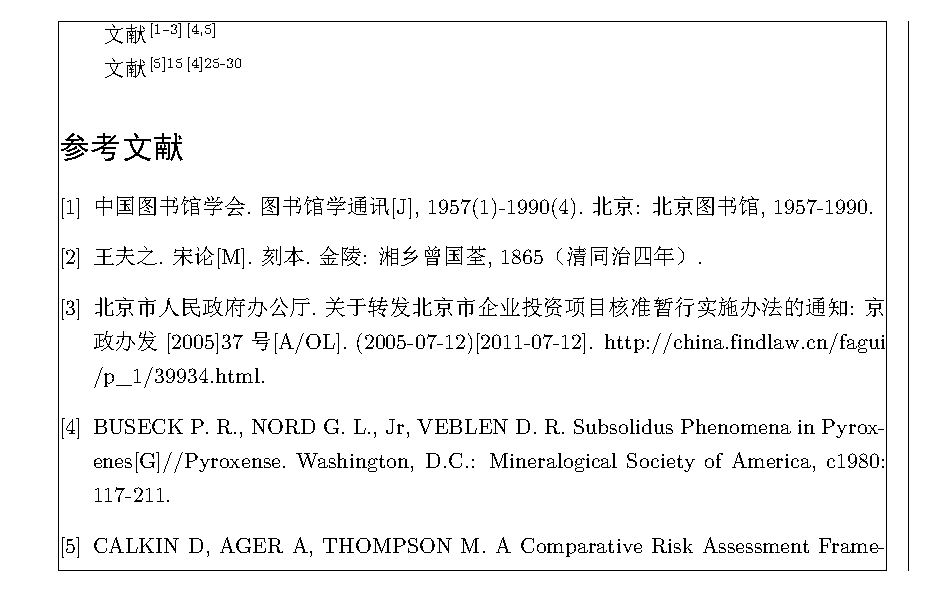
\includegraphics[width=0.9\linewidth]{example/egmwe.pdf}
\end{tcolorbox}
\caption{最小工作示例结果}\label{fig:usage:eg}
\end{figure}

更多示例见example文件夹内:

egmwe.tex 展示了一个最小工作示例;

egcitations.tex 展示了标注的命令;

egmulticitesty.tex 展示了局部化的标注样式;

egchapterbib.tex 展示了分章文献的用法。


文献表条目的格式化操作,由指定的样式文件设置,设置的方法详见下一小节。

\subsection{参考文献格式化设置说明}

参考文献格式化工作主要由bibmap程序结合样式文件来实现。bibmap程序主要实现的功能有:

1) 根据样式文件输出格式化后的bbl文件,便于latex文档直接使用。

2) 转存格式化的参考文献表文本为文本文件和网页文件,便于在其它文档中直接使用。

3) 除了bibmap程序内部处理逻辑外,样式文件可以全面控制参考文献的格式化。

4) bibmap实现的内部处理: 根据选项进行排序,根据选项对姓名列表域、文本列表域、日期域、文本域、范围域格式化,根据选项对条目输出项进行组织和格式化。

有时间进一步介绍内部处理逻辑的实现。

\subsubsection{样式文件的结构}

样式文件主要由几个字典参数构成,分别是:

\begin{description}
   \item[formatoptions] 用于设置格式化的全局选项,所设选项必须是bibmap程序支持的选项,主要包括:
       \begin{itemize}
       \item "style":写bbl信息的设置选项,authoryear,'numeric'
       \item "nameformat":'uppercase',\#姓名处理选项:uppercase,lowercase,given-family,family-given,pinyin
       \item "giveninits":'space',\#使用名的缩写,space表示名见用空格分隔,dotspace用点加空格,dot用点,terse无分隔,false不使用缩写
       \item "usesuffix":True,\#使用后缀名
       \item "maxbibnames":3,\#
       \item "minbibnames":3,\#
       \item "morenames":True,\#
       \item "maxbibitems":1,\#
       \item "minbibitems":1,\#
       \item "moreitems":False,\#
       \item "date":'year',\#'日期处理选项':year,iso,等
       \item "urldate":'iso',\#'日期处理选项':year,iso,等
       \item "origdate":'year',\#'日期处理选项':year,iso,等
       \item "eventdate":'year',\#'日期处理选项':year,iso,等
       \item 'caseformat':'none',\#设计'none','sentencecase','titlecase','uppercase','lowercase','smallcaps'
       \item 'numberformat':'ordinal',\#设计'ordinal','arabic'
       \item "lanorder":['chinese','japanese','korean','english','french','russian'],\# 文种排序,指定语言全面的顺序['chinese','japanese','korean','english','french','russian'],'none'
       \item 'sortascending':True,\#排序使用升序还是降序,默认是升序,设置为False则为降序
       \item "sorting":['author','year','title'],\#排序,或者指定一个域列表比如['key','author','year','title'],'none'
       \end{itemize}

   \item[localstrings] 用于设置本地化字符串,可以随意设置,只需符合规范。
   典型的设置方式为:
   \begin{example}{简单的localstrings参数设置}{code:usage:localstrings}
   \begin{pycode}
    #本地化字符串
    localstrings={
    'andothers':{'english':'et al.','chinese':'等'},
    'and':{'english':' and ','chinese':'和'},
    'edition':{'english':' ed','chinese':'版'},#ed. 中的点不要,为方便标点处理
    'in':{'english':'in: ','chinese':'见: '},
    'nolocation':{'english':'[S.l.]','chinese':'[出版地不详]'},
    'nopublisher':{'english':'[s.n.]','chinese':'[出版者不详]'},
    'bytranslator':{'english':'trans by','chinese':'译'},
    'volsn':{'english':'Vol.','chinese':'第'},
    'volume':{'english':'','chinese':'卷'},
    'numsn':{'english':'No.','chinese':'第'},
    'number':{'english':'','chinese':'册'},
    }
   \end{pycode}
   \end{example}

   \item[localpuncts] 用于设置标点,可以随意设置,只需符合规范。
   典型的设置方式为:
   \begin{example}{简单的localpuncts参数设置}{code:usage:localpuncts}
   \begin{pycode}
    #标点
    localpuncts={
    'multinamedelim':', ',
    'finalnamedelim':', ',
    'andothorsdelim':', ',
    'finalitemdelim':', ',
    'multiitemdelim':', ',
    'pagerangedelim':'-',
    }
   \end{pycode}
   \end{example}

   \item[replacestrings] 用于设置替换字符串,可以随意设置,只需符合规范。
   典型的设置方式为:
   \begin{example}{简单的replacestrings参数设置}{code:usage:replacestrings}
   \begin{pycode}
    #替换字符串
    replacestrings={
    '[出版地不详]: [出版者不详]':'[出版地不详 : 出版者不详]',
    '[S.l.]: [s.n.]':'[S.l. : s.n.]',
    '..':'.',
    }
   \end{pycode}
   \end{example}

   \item[typestrings] 用于设置类型和载体字符串,可以随意设置,只需符合规范。
   典型的设置方式为:
   \begin{example}{简单的typestrings参数设置}{code:usage:typestrings}
   \begin{pycode}
    #类型和载体字符串
    typestrings={
    'book':'[M]',
    'inbook':'[M]',
    'standard':'[S]',
    'periodical':'[J]',
    'article':'[J]',
    'newspaper':'[N]',
    'patent':'[P]',
    'online':'[EB]',
    'www':'[EB]',
    'electronic':'[EB]',
    'proceedings':'[C]',
    'inproceedings':'[C]',
    'conference':'[C]',
    'collection':'[G]',
    'incollection':'[G]',
    'thesis':'[D]',
    'mastersthesis':'[D]',
    'phdthesis':'[D]',
    'report':'[R]',
    'techreport':'[R]',
    'manual':'[A]',
    'archive':'[A]',
    'database':'[DB]',
    'dataset':'[DS]',
    'software':'[CP]',
    'map':'[CM]',
    'unpublished':'[Z]',
    'misc':'[Z]',
    }
   \end{pycode}
   \end{example}

   \item[datatypeinfo] 用于将条目的域进行分类,6个类型已经由bibmap程序设定,每一类域都有自身的特定处理逻辑。类型中包含的域可以由用户只有设定。
       典型的设置方式为:
   \begin{example}{简单的replacestrings参数设置}{code:usage:replacestrings}
   \begin{pycode}
    #数据类型
    datatypeinfo={
    'namelist':['author','editor','translator','bookauthor'],
    'literallist':['location','address','publisher','institution','organization','school','language','keywords'],
    'literalfield':['title','journaltitle','journal','booktitle','subtitle','titleaddon','url','doi','edition','version',
                    'volume','number','endvolume','endnumber','type','note','labelnumber','series'],
    'datefield':['date','enddate','year','endyear','urldate','origdate','eventdate','endurldate','endorigdate','endeventdate'],
    'rangefield':['pages'],
    'otherfield':['in','typeid','endpunct']#虚设的用于替换的域
    }
   \end{pycode}
   \end{example}


   \item[bibliographystyle]  用于设定条目的著录格式,用户可以自由设定。
    一个条目类型作为一个字典项,项值内容则表示该条目的域的组织顺序及其内容格式,每个域的设置格式构成一个域格式字典,域格式字典中的项可以使用bibmap提供的项,以实现需要的格式,项值设置,可以使用前述的任何设置,包括全局选项同名的选项,用于局部化设置。
    \begin{itemize}
    \item "fieldsource", 用于设置当前输出项的域名
    \item 'options',用于设置当前输出项的格式选项
    \item 'prepunct',用于设置当前输出项前的标点
    \item 'prepunctifnolastfield',用于设置当前输出项前的标点,仅在前一项不存在时输出
    \item "prestring",用于设置当前输出项前的字符串
    \item 'prestringifnumber',用于设置当前输出项前的字符串,仅当当前项为数字时输出
    \item 'replstring',用于设置替换当前输出项前的字符串
    \item "posstring",用于设置当前输出项后的字符串
    \item 'posstringifnumber',用于设置当前输出项后的字符串,仅当当前项为数字时输出
    \item "omitifnofield",用于忽略当前项,当该选项指定的域都不存在时,忽略当前项
    \item "omitiffield",用于忽略当前项,当该选项指定的域只要一个存在,则忽略当前项
    \item 'pospunct',用于设置当前输出项后的标点
    \end{itemize}

\end{description}

\subsubsection{样式文件的设置原理}

样式设置的核心在bibliographystyle参数,它设置了条目的域的顺序、域本身的格式、域前后的标点和字符串。所以如localstrings等其它参数都是为bibliographystyle参数服务的,也包括全局的选项。全局选项与localstrings的差别在于,它还在bibliographystyle没有设置局部选项的情况下使用。选项的优先级是bib文件中条目本身给出的选项优先于bibliographystyle设置中给出的选项,进一步优先于全局的选项。总的来说,格式设置选项分三级,第一级是bib文件中条目给出的选项,第二级是条目类型格式设置时给出的选项,第三级才是全局选项。

一个简单bibliographystyle参数设置如例\ref{code:usage:bibstyle}所示,其中设置了条目类型"misc"的著录格式,"book"等其他所有类型复用misc类型的格式,复用的方式很简单,就是把misc作为其它类型的键值,比如:\verb|"book":"misc"|。

misc类型的格式中,
第一项,输出的备选域包括作者,编者,译者,方式为:
\verb|"fieldsource":['author','editor','translator']|,
因为这是姓名列表类型的域,给它指定了条目类型一级的选项:
\verb|'options':{'nameformat':'uppercase'}|,意为姓名采用全大写字母的格式。

第二项,输出的备选域为标题,方式为:
\verb|"fieldsource":['title']|;
因为这是文本类型的域,给它指定了给它指定了条目类型一级的选项:

\verb|'options':{'caseformat':'sentencecase'}|,意为标题采用句子模式的大小写格式;
另外设置了前置标点,前一项不存在时输出的标点,后置的字符串,方式为:

\verb|'prepunct':". ",'prepunctifnolastfield':'','posstring':r"\allowbreak\typestring"|
其中默认前置标点为一个点加空格,当前一项不存在时则标点变为空,后置一个字符串中加入了
\verb|\allowbreak|命令,以及一个\verb|\typestring|,\verb|\typestring|最后会根据typestrings参数的设置替换为对应的字符串,
若typestrings设置如例\ref{code:usage:typestrings}所示,那么\verb|\typestring|会替换为[z]。

第三项,输出的备选域为'howpublished',方式为:
\verb|"fieldsource":['howpublished']|;
仅设置了一个前置标点为点加空格:
\verb|'prepunct':". "|。

第四项,输出的备选域为地址,location和address都表示地址,有时会混用,所以两者都给出,方式为:
\verb|"fieldsource":['location','address']|;
仅设置了一个前置标点为点加空格:
\verb|'prepunct':". "|。

第五项,输出的备选域为出版者,institution和publisher都可以表示出版者,有时会混用,所以两者都给出,方式为:
\verb|"fieldsource":['institution','publisher']|;
设置了一个前置标点为冒号加一个空格,当前一项即地址项不存在时则输出标点为点加空格:
\verb|'prepunct':": ",'prepunctifnolastfield':'. '|。

第六项,输出的备选域为日期,'date'和'year'都可以表示日期,有时会混用,所以两者都给出,方式为:
\verb|"fieldsource":['date','year']|;
设置了一个前置标点为逗号加一个空格:
\verb|'prepunct':", "|。

第七项,输出的备选域为页码,方式为:
\verb|"fieldsource":['pages']|;
设置了一个前置标点为冒号加一个空格:
\verb|'prepunct':": "|。

第八项,输出的备选域为网址访问日期,方式为:
\verb|"fieldsource":['urldate']|;
设置了一个前、后字符串为方括号,目的是把访问日期用方括号包围起来:

\verb|'prestring':"[","posstring":"]"|。

第九项,输出的备选域为网址,方式为:
\verb|"fieldsource":['url']|;
设置了一个前置标点为点加空格,前置字符串为一个newblock命令和url命令和花括号,后置字符串为花括号。目的是把网址包围在url命令内:

\verb|'prepunct':r". ",'prestring':r'\newblock\url{','posstring':'}'|。

第十项,输出的备选域为doi,方式为:
\verb|"fieldsource":['doi']|;
设置了一个前置标点为点,前置字符串为一个newblock命令加DOI:和url命令和花括号,后置字符串为花括号。目的是把网址包围在url命令内:

\verb|'prepunct':".",'prestring':r'\newblock DOI:\doi{','posstring':'}'|。

最后一项是,虚设的域endpunct,目的就是用来做替换。这里将其替换为一个点。方式为:
\verb|{"fieldsource":['endpunct'],'replstring':"."}|。

\begin{example}{简单的bibliographystyle参数设置}{code:usage:bibstyle}
\begin{pycode}
#条目的著录格式
bibliographystyle={
"misc":[
{"fieldsource":['author','editor','translator'],'options':{'nameformat':'uppercase'}},
{"fieldsource":['title'],'options':{'caseformat':'sentencecase'},'prepunct':". ",'prepunctifnolastfield':'','posstring':r"\allowbreak\typestring"},
{"fieldsource":['howpublished'],'prepunct':". "},
{"fieldsource":['location','address'],'prepunct':". "},
{"fieldsource":['institution','publisher'],'prepunct':": ",'prepunctifnolastfield':'. '},
{"fieldsource":['date','year'],'prepunct':", "},
{"fieldsource":['pages'],'prepunct':": "},
{"fieldsource":['urldate'],'prestring':"[","posstring":"]"},
{"fieldsource":['url'],'prepunct':r". ",'prestring':r'\newblock\url{','posstring':'}'},
{"fieldsource":['doi'],'prepunct':".",'prestring':r'\newblock DOI:\doi{','posstring':'}'},
{"fieldsource":['endpunct'],'replstring':"."}
],
"book":"misc",
"article":"misc",
"newspaper":"misc",
"inbook":"misc",
"inproceedings":"misc",
"incollection":"misc",
"proceedings":"misc",
"collection":"misc",
"standard":"misc",
"patent":"misc",
"online":"misc",
"www":"misc",
"electronic":"misc",
"report":"misc",
"techreport":"misc",
"periodical":"misc",
"thesis":"misc",
"manual":"misc",
"unpublished":"misc",
"database":"misc",
"dataset":"misc",
"software":"misc",
"map":"misc",
"archive":"misc",
"phdthesis":"misc",
"mastersthesis":"misc",
}
\end{pycode}
\end{example}

例\ref{code:usage:bibstyle}给出的参考文献著录格式,仅对misc类型做了设置,其它类型全部复用该类型的格式。如果要对其它类型做更专门的设置,可以采用类似misc的方式进行设置。宏包提供的bibstylenumeric.py 样式文件就是精确实现国标要求的设置。

需要注意的是,bibliographystyle参数设置格式,主要设置各输出项所用的域,以及标签,前后添加的字符串等。而域内容本身的格式,则由bib文件中条目本身提供的选项、各输出项设置时给出的条目类型一级的选项,以及formatoptions参数给出的全局选项控制。格式在bibmap程序中实现,不同类型的域实现逻辑不同。主要分为:
    'namelist'(姓名列表域,用于处理姓名列表,姓名成分解析和姓名格式化)、
    'literallist'(文本列表域,用于处理文本列表,解析和格式化)、
    'literalfield'(文本列表域,包含字符串、数字域等,有数字序号、字母大小写等处理)、
    'datefield'(日期域,用于处理日期和日期范围,日期成分解析和日期格式化)、
    'rangefield'(范围域,主要是页码域,处理页码间隔符)、
    'otherfield'(虚设域用于替换)。
各个域的处理逻辑在bibmap程序中实现,用户可以控制部分,都可以通过三个层级的选项来进行控制。

\section{bib文件修改的详细说明}

\subsection{bib文件修改示例}

bib文件修改功能主要有如下几个:

1) bib文件的读取和解析

2) bib文件的转存,包括从大的bib文件抽取引用的文献保存为一个小的bib文件,将bib文件的内容存储为json格式的问题。

3) 参考文献条目的修改,包括条目类型的修改,条目内部的域的修改等,包括删除、变化、转换等等。

修改的逻辑是bibmap程序读取数据修改样式文件内的sourcemaps参数,这个sourcemaps参数与biblatex中sourcemap非常像,基本的逻辑也是一样的,只是把tex的写法转换成了python方便表示的写法,就是把biblatex用tex命令表示的\verb|\maps|、\verb|\map|和\verb|\step|转换为用json格式表示。sourcemaps参数的设置方法见下一节。


\subsection{bib文件修改设置说明}

\subsubsection{数据修改样式文件的结构}

数据修改样式文件是一个py文件,内部但要保存一个或多个sourcemaps参数,但要注意虽然可以存在多个sourcemaps,但后面的sourcemaps会覆盖前面的sourcemaps,也就是只有最后一个sourcemaps会起作用。

典型设置如例\ref{code:usage:mapstyle}所示,其中sourcemaps是一个列表参数,包含了所有map步骤,每个map也是一个列表,一个map就是对所有条目进行一次遍历修改。一个map列表中包含有任意数量的step(步骤),一个step是由一个key-val参数构成字典数据结构。数据的修改是由step步的key-val参数字典决定的。

简单来说,数据修改逻辑是这样的,bibmap程序读取sourcemaps参数后,开始遍历所有的map,
这一个map处理需要遍历所有的bib条目,对于每个条目,遍历当前map内的所有step步,step步的执行规则由step步内的参数以及处理结果确定。

\begin{example}{bib数据修改的处理逻辑}{code:usage:maplogic}
\begin{pycode}
	for map in maps #遍历maps中的所有map
		for entry in entries #对所有的条目均执行该map
			for step in map #遍历map中的所有step
				code for the step to modify the bib entry	
\end{pycode}
\end{example}

例\ref{code:usage:mapstyle}给出了10次map的数据修改。

第一次修改,内部只有一个step步,目的是将ELECTRONIC类型转换为online类型:

\verb|{"typesource":"ELECTRONIC","typetarget":"online"}|。

其中使用了键typesource和typetarget,意为将类型为typesource值的条目,转换为typetarget值的类型。比如这里将ELECTRONIC类型条目转换为online条目。

第二次修改,内部只有一个step步,目的是将source域转换为url域:

\verb|{"fieldsource":"source","fieldtarget":"url"}|

其中使用了键fieldsource和fieldtarget,意为将条目中域名为fieldsource值的域,转换为名为fieldtarget值的域。比如这里将source域转换为url域。

第三次修改,内部只有一个step步,目的是将urldate域的信息“yyyy-m-d”转换为“yyyy-mm-dd”便于日期能够正常解析。

\verb|{"fieldsource":"urldate","match":r'(\d\d\d\d)\-(\d)\-(\d)',"replace":r'\1-0\2-0\3'}|

其中使用了键fieldsource、match、replace,意为对条目中域名为fieldsource值的域做匹配,当匹配到match键的值时,将匹配内容体会为replace键的值。这里的匹配和替换可以使用普通的字符串,也可以使用正则表达式,这里就是使用的正则表达式。但是要注意一旦涉及到已经存在的域内容的修改,都需要选项overwirte的支持,也就是要加上overwrite键。就是说,这次修改实际不会执行,而下一次的修改,由于overwrite存在才会执行。

第四次修改,基本同第三次修改,由于overwrite键设置为true,则修改会实际执行:

\verb|{"fieldsource":"date","match":r'(\d\d\d\d)\-(\d)\-(\d)',"replace":r'\1-0\2-0\3',"overwrite":True}|

第五次修改,类似于第二次修改,将refdate域转换为urldate域:

\verb|{"fieldsource":"refdate","fieldtarget":"urldate"}|

第六次修改,内部有2个step步,目的是为newspaper类型的条目,设置note域为news。

第一步为:
\verb|{"pertype":"newspaper"}|,是做了条目类型约束,pertype键表示只有其键值给出的条目类型才做修改。

第二步为:

\verb|{"fieldset":"note","fieldvalue":"news","overwrite":True}|

使用了键包括fieldset、fieldvalue、overwrite。fieldset表示对其值表示的域做修改,fieldvalue就是修改后的值,overwrite表示域有原内容的情况下做覆盖修改。若不该处overwrite,那么当note域原来就存在情况下,当前步不实际执行。

第七次修改,内部有2个step步,目的是设置edition域等于version。

第一步为:
\verb|{"fieldsource":"version","final":True}|

是做域查找,当条目中version存在时,并记录version的域值。final键的目的是,当条目中不存在version域时,本次map直接终止,即后面的step步不再执行。

第二步为:

\verb|{"fieldset":"edition","origfieldval":True}|


使用了键包括fieldset、origfieldval。fieldset去设置edition域,域的值为origfieldval表示的内容,即前面一步fieldsource查找并记录下的version域的值。origfieldval表示前面的最近一步fieldsource记录下的域值信息。

第八次修改,与第七次类似,目的是将entrykey域的内容设置给keywords域。

第九次修改,与第七次类型,目的是对于存在note域的情况,将其值添加到keywords。需要注意的是第二步中,使用了append键,目的是修改过程中,不是覆盖修改,而是做添加修改。overwrite键也需要给出,否则无法对已经存在的域做修改。

第二步设置为:
\verb|{"fieldset":"keywords","origfieldval":True,"overwrite":True,"append":True}|

第十次修改,内部由两个step步,目的是根据标题的字符编码范围确定标题的语言类型。

第一步:
\verb|{"fieldsource":"title","match":r'[\u2FF0-\u9FA5]',"final":True}|

目的是搜索fieldsource指出的title域,是否匹配match指出的正则表达式,当不能匹配时,根据final键,直接终止当前map,即第二步step不再处理。

第二步:
\verb|{"fieldset":"userd","fieldvalue":"chinese"}|

目的是,当前一步匹配成功,那么将当前条目的userd域设置为fieldvalue指出的值即chinese。


\begin{example}{典型的bib数据修改样式参数设置}{code:usage:mapstyle}
\begin{pycode}
#
#数据修改的设置
#
#
# 为数据map设置参数
# 选项的逻辑与biblatex基本一致,
# 差别包括:overwrite选项可以放到step步中表示
#[]=maps
#[[],[]]=map in maps
#[[{optionkey:optionval},{optionkey:optionval}],[]]=step in map in mpas
#注意python正则表达方式与perl的略有不同,比如unicode表示
#python用\xHH,\uHHHH,\UHHHHHHHH表示,而perl直接用\x{HHHH}表示。
sourcemaps=[#maps
	[#map1:将ELECTRONIC类型转换为online类型
		{"typesource":"ELECTRONIC","typetarget":"online"}#step1
	],
	[#map2:将source域转换为url域
		{"fieldsource":"source","fieldtarget":"url"}#step1
	],
	[#map3:将urldate域的信息“yyyy-m-d”转换为“yyyy-mm-dd”,注意正则表达式直接写不用在外面套""
		{"fieldsource":"urldate","match":r'(\d\d\d\d)\-(\d)\-(\d)',"replace":r'\1-0\2-0\3'}#step1
	],
	[#map4:将urldate域的信息“yyyy-m-d”转换为“yyyy-mm-dd”,注意正则表达式直接写不用在外面套""
		{"fieldsource":"date","match":r'(\d\d\d\d)\-(\d)\-(\d)',"replace":r'\1-0\2-0\3',"overwrite":True}#step1
	],
	[#map5:将refdate域转换为urldate域
		{"fieldsource":"refdate","fieldtarget":"urldate"}#step1
	],
	[#map6:对于newspaper类型,设置note为news
		{"pertype":"newspaper"},#step1
		{"fieldset":"note","fieldvalue":"news","overwrite":True}#step2
	],
	[#map7:设置edition域等于version
		{"fieldsource":"version","final":True},#step1
		{"fieldset":"edition","origfieldval":True}#step2
	],
	[#map8:设置entrykey域设置给keywords
		{"fieldsource":"entrykey"},#step1
		{"fieldset":"keywords","origfieldval":True}#step2
	],
	[#map9:对于存在note域的情况,将其值添加到keywords
		{"fieldsource":"note","final":True},#step1
{"fieldset":"keywords","origfieldval":True,"overwrite":True,"append":True}#step2
	],
	 [#map10:根据标题的字符编码范围确定标题的语言类型
		{"fieldsource":"title","match":r'[\u2FF0-\u9FA5]',"final":True},#step1
		{"fieldset":"userd","fieldvalue":"chinese"}#step2
	],
]
\end{pycode}
\end{example}


例\ref{code:usage:mapstyle}大体上给出了数据修改参数设置的方法,下一节详细介绍一下bibmap支持的键。

\subsubsection{数据修改支持的选项}

bibmap数据修改所用的选项,即各step步中的key值,完全借鉴biblatex中的设计,其意义也是一致的,根据常用程度做了取舍,并增加了部分选项如fieldfunction,实现的选项包括:

\begin{itemize}
  \item typesource 对应的值为 entrytype名
  \item typetarget 对应的值为 entrytype名
  \item fieldsource 对应的值为 entryfield名
  \item fieldtarget 对应的值为 entryfield名
  \item match 对应的值为 regexp(正则表达式)
  \item notmatch 对应的值为 regexp(正则表达式)
  \item replace 对应的值为 regexp(正则表达式)

  \item notfield 对应的值为 entryfield名
  \item final 对应的值为 true和false(bool值)
  \item origfieldval 对应的值为 true, false(bool值)
  \item append 对应的值为 true, false(bool值)
  \item pertype 对应的值为 entrytype名即条目类型
  \item pernottype 对应的值为 entrytype名即条目类型

  \item fieldset 对应的值为 entryfield名
  \item fieldvalue 对应的值为 string(字符串)
  \item null 对应的值为 true, false(bool值)
  \item origfield 对应的值为 true, false(bool值)
  \item origentrytype 对应的值为 true, false(bool值)
  \item origfieldval 对应的值为 true, false(bool值)
  \item fieldfunction 对应的值为用户指定的函数名,目前提供的函数主要是:sethzpinyin。在 在域内容处理是,当给出'fieldfunction':'sethzpinyin'选项时,程序会调用sethzpinyin函数以域内容为参数,输出其对应的拼音。
\end{itemize}

其中绝大部分在前一节以及讲过,未介绍的包括notmatch与match类型,只是搜索的是不匹配的情况。
notfield是做约束,当notfield指出的域不存在时,才执行操作,通常和final联用。
pernottype类似于pertype,也是做约束,当不是pernottype指定的条目类型时,才执行操作。
null表示域值不存在,即用于删除当前域。origfield用于标签前面step步中最后一次fieldsource搜索并记录下的域的域名,而origfieldval则是域值。origentrytype则是前面最近一次typesource搜索成功情况下记录下来的条目类型。

未实现的选项包括:
\begin{itemize}
  \item entryclone=?clonekey?
  \item entrynew=?entrynewkey?
  \item entrynewtype=?string?
  \item entrytarget=?string?
  \item entrynocite=true, false default: false
  \item entrynull=true, false default: false
  \item matchi=?regexp?
  \item notmatchi=?regexp?
\end{itemize}
未实现的主要是条目整体复制和处理相关的内容,以及区分字符大小写的正则匹配。


\section{bibmap程序命令行用法}

\subsection{bibmap程序输入参数}

bibmap.py或bibmap.exe

filename 单个输入文件的文件名,可带后缀名如bib或aux,无后缀名时默认为辅助文件.aux

[-h] 输出帮助

[-a AUXFILE] 辅助文件的文件名,可带后缀名.aux,如果filename已经设置aux文件则无效

[-b BIBFILE] 文献数据库文件名,可带后缀名.bib,如果filename已经设置bib文件则无效

[-s STYFILE] 设置文献样式文件的文件名,可带后缀名.py,不给出则使用默认样式文件

[-m MAPFILE] 数据库修改设置文件文件名,可带后缀名.py,不给出则使用默认设置文件

\verb|[--addpinyin]| 给出该选项则将为每个文献条目增加带有拼音的key域。

\verb|[--nofmt]| 给出该选项则不做格式化输出

\verb|[--nobdm]| 给出该选项则不做bib数据修改

其中涉及到三种文件:

一是aux文件,如果是要得到格式化的文献表,那么这是最重要的文件,由tex编译生成,当使用bibmap宏包时,可以通过宏包选项设置样式文件,而bib文件通过bibliography命令也会在该文件中指出。

二是bib文件,这是参考文献数据源文件,可以由通过bibliography命令在aux文件内给出,也可以直接利用选项给出。

三是py文件,这是用于设置数据修改和文献格式化的文件,是python代码。宏包自带的样式,通常bibmap*.py是用于bib文件数据修改的,而bibstyle*.py是用于格式化文献表的。



\subsection{bib文件数据修改}

直接在命令行输入脚本及其参数:

\begin{example}{bib文件数据修改命令-默认情况}{code:bib:modify}
\begin{pycode}
python bibmap.py biblatex-map-test.bib
或
bibmap.exe biblatex-map-test.bib
\end{pycode}
\end{example}

此时,bibmap读取biblatex-map-test.bib文件,并根据默认的数据修改设置bibmapdefault.py做修改,此时还会自动的做格式化后的文献表输出。

\begin{example}{bib文件数据修改命令-不输出格式化文献表}{code:bib:modifya}
\begin{pycode}
python bibmap.py biblatex-map-test.bib --nofmt
或
bibmap.exe biblatex-map-test.bib  --nofmt
\end{pycode}
\end{example}

此时不再输出格式化后的文献表。

\begin{example}{bib文件数据修改命令-指定数据修改设置}{code:bib:modifyb}
\begin{pycode}
python bibmap.py biblatex-map-test.bib --nofmt -m bibmapaddkw.py
或
bibmap.exe biblatex-map-test.bib --nofmt -m bibmapaddkw.py
\end{pycode}
\end{example}

此时使用指定的数据修改设置bibmapaddkw.py代替默认的bibmapdefault.py对数据库bib文件做修改。


又比如给中文的参考文献条目增加带有拼音的key域,可以采用如下方式:
\begin{example}{bib文件数据修改命令-增加拼音信息的key域}{code:bib:addpinyin}
\begin{pycode}
bibmap.exe  biblatex-map-test.bib --nofmt --addpinyin
或
bibmap.exe biblatex-map-test.bib --nofmt -m bibmapaddpinyinkey.py
或
python bibmap.py biblatex-map-test.bib --nofmt --addpinyin
或
python bibmap.py biblatex-map-test.bib --nofmt -m bibmapaddpinyinkey.py
\end{pycode}
\end{example}




\subsection{参考文献格式化输出}

直接在命令行输入脚本及其参数:

\begin{example}{参考文献格式化命令-默认情况}{code:bib:fmt}
\begin{pycode}
python bibmap.py egtest
或
bibmap.exe egtest
\end{pycode}
\end{example}

此时输入一个辅助文件egtest.aux,其它所有的参数根据对egtest.aux的解析来获取,如果没有解析到,若存在默认的设置,则使用默认的设置文件。若没有默认设置,则可以通过可选参数来指定:

\begin{example}{参考文献格式化命令-指定bib文件}{code:bib:fmta}
\begin{pycode}
python bibmap.py egtest -b biblatex-map-test.bib
或
bibmap.exe egtest -b biblatex-map-test.bib
\end{pycode}
\end{example}

当aux文件未给出格式化设置文件时,也可以用-s选项给出,格式化设置文件(即文献样式文件),比如
\begin{example}{参考文献格式化命令-指定样式文件}{code:bib:fmta}
\begin{pycode}
python bibmap.py egtest -s bibstyleauthoryear.py
或
bibmap.exe egtest -s bibstyleauthoryear.py
\end{pycode}
\end{example}


\section{结论}

本宏包最初的工作,只是想设计一个python脚本,方便对bib文件进行修改,而不去使用bib管理软件或者使用biber程序(biber 做bib修改需要tex文件支持,因而为修改bib必须写一个tex文件)。做到一定程度后,本想为biblatex-check脚本做个pr了事,但没想到又接着写下去了,慢慢变成了两个主要功能,一是参考文献bib文件数据修改,二是参考文献格式化,既便于bib文件的修改、转换和保存,也便于格式化后直接给latex应用或者文本复制和网页显示。第二个功能整体上已经类似于bibtex,所以也就继续完善下来,最终形成了目前的bibmap宏包。基于传统的参考文献生成方法,利用natbib等现成宏包,替代bibtex程序,形成一个便于参考文献生成的程序和宏包。

目前功能已经大体实现,欢迎大家使用,并提出各方面的意见建议!

值得说明的是,sty文件中标注命令相关内容,详细参考了gbt7714宏包和ucas-thesis模板,部分代码直接借用,对其作者Lee Zeping 和 Mo Huangrui表示由衷的感谢!

\clearpage
\appendix

因为bibmap宏包的标注样式基于natbib宏包实现,而要使用分章的参考文献,那么需要使用chapterbib宏包,因此对这两个宏包做一些介绍方便使用。

\section{natbib宏包用法简介}

\subsection{基本概念}

natbib宏包主要用来生成标注标签,在不同的章节可以使用不同的标注样式。

\subsection{用法和注意事项}

1. 当与chapterbib联用时,sectionbib选项需要在natbib宏包加载时给出。给chapterbib设置无效。

2. 文献表的样式仍然设置用\verb|\bibliographystyle{}|命令。

3. natbib提供了常用的citet和citep命令,通常citet会提供作者信息,citep会加上包围的符号。当然在natbib加载不同的选项时,会有不同的表现。

4. natbib提供了三个plainnat.bst abbrvnat.bst unsrtnat.bst样式文件。

5. thebibliography环境的语法:

\verb|\bibitem[Jones et al.(1990)]{jon90}...|

或

\verb|\bibitem[Jones et al.(1990)Jones, Baker,and Williams]{jon90}...|

其中(年份)前的是缩略的姓名列表。后面的则是详细的列表。该列表在首次引用需要详细姓名的样式中会用到。

6. 提供了大量的cite类命令,可以输出作者,年份,数字等信息。可以大小写变化。这些按需使用,最常用的还是前面提过的citet和citep。

7. 还可以利用\verb|\defcitealias|命令定义别名标签,某些情况下要生成特定的标签会非常有用。

8. 可以利用\verb|\setcitestyle|命令来局部设置标注的样式,该命令的参数是key=val或key结构。
也可以利用\verb|\bibpunct|命令来设置标注的样式,主要是标点。
也可以利用\verb|\bibstyle@xxx|命令来预设置一种标注样式,然后用\verb|\citestyle|命令来使用。

比如:
\verb|\newcommand{\bibstyle@agu}{\bibpunct{[}{]}{;}{a}{,}{,~}}|

然后使用:
\verb|\citestyle{agu}|

natbib已经预定义的样式包括:
plain、
plainnat、
agu、
egu、
agms、
cospar、
nature。

setcitestyle, bibpunct, citestyle 的设置的样式会覆盖宏包加载时的样式。

9. 可以使用如下命令进一步格式化:

\verb|\bibsection|
\verb|\bibpreamble|
\verb|\bibfont|
\verb|\citenumfont|
\verb|\bibnumfmt|
\verb|\bibhang|
\verb|\bibsep|

10. 标注的排序和压缩,使用sort\&compress 选项。

11. 顺序编码样式中的,分组引用,可以使用merge选项,然后使用*来构成分组。比如:
\verb|\citep{feynmann,*salam,*epr}|会形成一个数字。

12. 作者年制中的长标注,比如第一次引用时,使用长标注。可以使用\verb|\citet*|等命令。

13. 常用选项包括:

round (default) for round parentheses;

square for square brackets;

curly for curly braces;

angle for angle brackets;

semicolon (default) to separate multiple citations with semi-colons;

colon the same as semicolon, an earlier mistake in terminology;

comma to use commas as separators;

authoryear (default) for author{year citations;

numbers for numerical citations;

super for superscripted numerical citations, as in Nature;

sort orders multiple citations into the sequence in which they appear in the list of references;

sort\&compress as sort but in addition multiple numerical citations are compressed if possible (as 3{6, 15);

compress to compress without sorting, so compression only occurs when the given citations would produce an ascending sequence of numbers;

longnamesfirst makes the first citation of any reference the equivalent of the starred variant (full author list) and subsequent citations normal (abbreviated list);

sectionbib redefines thebibliography to issue section* instead of chapter*; valid only for classes with a chapter command; to be used with the chapterbib package;

nonamebreak keeps all the authors’ names in a citation on one line; causes
overfull hboxes but helps with some hyperref problems;

merge to allow the * prefix to the citation key, and to merge such a citation’s reference with that of the previous citation;

elide to elide common elements of merged references, like the authors or year;
mcite to recognize (and ignore) the merging syntax

14. 注意:当出现unskip命令不能出现在竖直环境中的错误时,说明引用命令没有进入水平模式,只要在引用命令前加上文本即可。


\section{chapterbib宏包用法简介}

\subsection{基本概念}
分章文献的基本原理是利用include,来对不同的章生成不同的aux文件,然后对各个aux文件信息仅需解析,然后处理bib文件,进而生成多个bbl文件即多个thebibliography环境,进而可以生成多个文献表。

因此对于利用bibtex处理bib文件的方法,每个文件中必须要\verb|\bibliographystyle| 和 \verb|\bibliography|命令指出相应的bst样式和bib文件。才能让bibtex读取每个aux文件时获取足够的信息。

chapterbib也提供了cbunit和\verb|\cbinput|命令,可以不基于include方法来生成多个文献表。但是这种方法需要比较麻烦的编译过程,所以不推荐使用。

\subsection{用法和注意事项}

1. 在book和report类中,参考文献的标题会被当做是一个chapter*的标题,但若要使得参考文献的标题降一个层级,比如降到section*。那么可以使用sectionbib选项,但与natbib连用时,该选项会失效,替代的方法是给natbib设置这个选项。


2. 要在主文档中使用一个完全不同的参考文献,那么不能再使用\verb|\bibliography|命令,因为主文档bbl会包含值文档的。所以只能使用手写的thebibliography环境。

3. 要在主文档生成一个包含所有子文档文献的文献表,那么可以使用\verb|\bibliography|命令。而要避免报错,\verb|\bibliographystyle| 必须要放在所有的include之前。或者也可以在不同的编译步使用或不使用[rootbib]选项来实现。

4. 要把所有各章的文献表收集起来放到主文档中,那么可以使用[gather]选项,然后在主文档中使用
\verb|bibliography|命令。也可以通过定义\verb|\StartFinalBibs|来重定义文献表的标题。

5. 如果文献表不仅要收集起来,也需要在各章显示,那么可以使用[duplicate]选项。



\end{document}
